\documentclass[12pt,a4paper]{article}
\usepackage[utf8]{inputenc}
\usepackage[T1]{fontenc}
\usepackage{amsmath}
\usepackage{xcolor}
\usepackage{color}
\usepackage{pifont}
\everymath{\displaystyle}
\usepackage[francais]{babel}
\usepackage{fancyhdr}
\usepackage{fancybox}
\usepackage{hyperref}
\usepackage{graphicx}
\usepackage{wrapfig}

\usepackage{fancyhdr}
\usepackage[left=1.3cm,right=1.2cm,top=2cm,bottom=1.5cm]{geometry}
\usepackage{array}
\pagestyle{fancy}
\fancyhead[L]{Florentin Lespinasse~~~~~~~~~~~~~~~1STI2D4}
\fancyhead[C]{~~~~~~~~~~~~~~~~~~~~~~~~~~~Devoir Maison}
\fancyhead[R]{Enero 8, 2020}
\colorlet{darkgreen}{green!50!black}

\begin{document}
\begin{center}
        \shadowbox{\begin{large}
                \textcolor{black}{Robots y Humanos}
        \end{large}}
    \end{center}
    \vspace{0.5 cm}
\begin{center}
\textcolor{darkgreen}{\textit{\textbf{Objectivo :}} Explicar la relaci\'on entre inteligencia artificial e inteligencia humana.}
\end{center}

\begin{wrapfigure}[7]{l}{5.5cm}
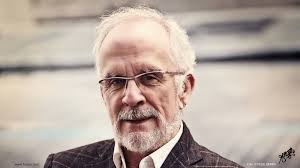
\includegraphics[scale=0.5]{Antonio.jpeg}
\end{wrapfigure}

\begin{partie1}
\noindent \large 1) Describe lo que ves en la vi\~neta. Identifica a los personajes del dibujo indicando de qu\'e hablan.  \par 
	\normalsize En la vi\~neta, hay un humano que camina en la carretera con su perro. 
	Hay tambi\'en el perro que pensa. \\
	El humano habla de los Fan\'aticos que robado la compation y el perro dice que este humano tiene razon, que la compasion este a los perros.\\

\end{partie1}

\begin{partie2}
\noindent \large 2) A tu parecer, ¿Por qu\'e Forges eligi\'o esta relaci\'on due\~nos-perro para abordar este tema? \par
	\normalsize Forges eligi\'o este relation porque es la relaci\'on el mas fuerte. 
	Los perros ha muchos compasion comparado a los humanos.
	Un due\~no debe hace cuidado su compa\~neros. \\
	

\end{partie2}

\begin{partie3}
\noindent \large 3) Explica lo que quiere denunciar el dibujante.  \par
	\normalsize Este vi\~neta denoncia que los inhumano ha no sentimentos.
	Que los humano tamb\'ien pero han un poco. 
	Los perros han muchos sentimentos.
	Este autor denoncia tamb\'ien la violencia del intolerancia.

\end{partie3}


\end{document}

